\documentclass{standalone}
\usepackage{tikz}
\usepackage{amsmath}
\usepackage{lmodern}
\usepackage{pgfplots}
\pgfplotsset{compat=1.17}

\begin{document}

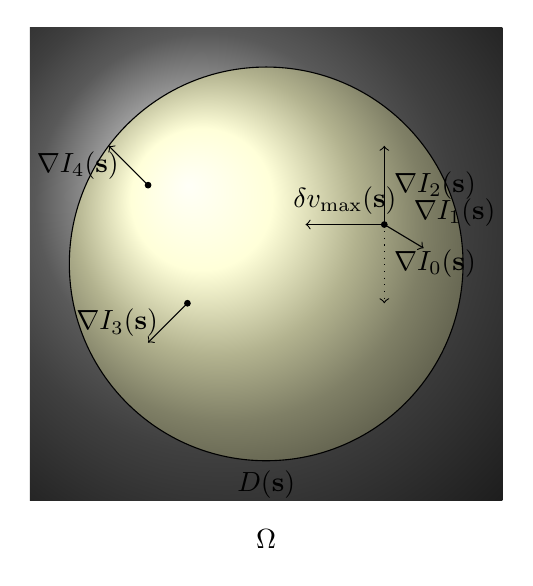
\begin{tikzpicture}

% Define colors
\definecolor{myGradientStart}{rgb}{1,1,0.8}
\definecolor{myGradientEnd}{rgb}{0.5,0.5,0.5}

% Background gradient
\fill[ball color=myGradientEnd] (-3,-3) rectangle (3,3);

% Circle with gradient
\shade[ball color=myGradientStart] (0,0) circle (2.5);

% Main circle
\draw (0,0) circle (2.5);

% Labels and vectors
\filldraw (1.5,0.5) circle (1pt);
\draw[->] (1.5,0.5) -- (0.5,0.5) node[midway, above] {$\delta v_{\max}(\mathbf{s})$};
\draw[->] (1.5,0.5) -- (1.5,1.5) node[midway, right] {$\nabla I_2(\mathbf{s})$};
\draw[->, dotted] (1.5,0.5) -- (1.5,-0.5) node[midway, right] {$\nabla I_0(\mathbf{s})$};
\draw[->] (1.5,0.5) -- (2.0,0.2) node[midway, above right] {$\nabla I_1(\mathbf{s})$};

\filldraw (-1,-0.5) circle (1pt);
\draw[->] (-1,-0.5) -- (-1.5,-1) node[midway, left] {$\nabla I_3(\mathbf{s})$};

\filldraw (-1.5,1) circle (1pt);
\draw[->] (-1.5,1) -- (-2,1.5) node[midway, left] {$\nabla I_4(\mathbf{s})$};

% Circle label
\node at (0,-2.8) {$D(\mathbf{s})$};

% Outer label
\node at (0,-3.5) {$\Omega$};

\end{tikzpicture}

\end{document}